\Introduction
\label{ch:introduction}

L'informatique graphique, branche du domaine de l'informatique, est l'étude de la création d'images numériques par ordinateur~\cite{poinssac_infographie_1994}. C'est un domaine à l'intersection de plusieurs disciplines, comme l'informatique, les mathématiques, la physique, l'optique, la biologie, et d'autres encore. L'informatique graphique trouve ses applications dans de nombreux autres domaines \footnote{\og When Did 3D Modeling Start? A Brief History \fg, 2021, Sammy Ekaran, accès le 20 décembre 2023, \url{https://www.selfcad.com/blog/when-did-3d-modeling-start-a-brief-history}}, notamment celui du divertissement. Un défi de l'informatique graphique qui se dresse depuis ses débuts est celui de la création de contenu, car c'est un processus long et coûteux. Dans la figure~\ref{fig:hades} par exemple, le personnage, les bâtiments et leur architecture, la rivière et les effets de lumières sont tous des éléments créés par une équipe d'artistes. Il existe diverses méthodes pour créer du contenu \footnote{\og Why 3D Modeling Is Important in Gaming Industry? \fg, 2023, Juegoadmin, accès le 20 décembre 2023, \url{https://www.juegostudio.com/blog/why-3d-modeling-is-important}}, dont plusieurs comme le modelage 3D, qui demandent beaucoup de temps de travail aux artistes. De nos jours en particulier, il y a une demande croissante pour des univers virtuels de plus en plus grands et détaillés \footnote{\og Open World Gaming : From a few titles to an industry standard \fg, 2022, Amir Imam, accès le 21 décembre 2023, \url{https://renderwonk.com/publications/s2010-shading-course/hoffman/s2010_physically_based_shading_hoffman_a_notes.pdf}}. Les méthodes traditionnelles de création de contenu, par le pur travail manuel des artistes, sont de moins en moins viables en raison de la quantité de contenu nécessaire à créer pour remplir ces univers~\cite{freiknecht_survey_2017}. Il est important de mettre au point des méthodes plus automatisées pour permettre une création plus rapide et moins coûteuse.

\bigskip

\begin{figure}[!h]
    \centering
    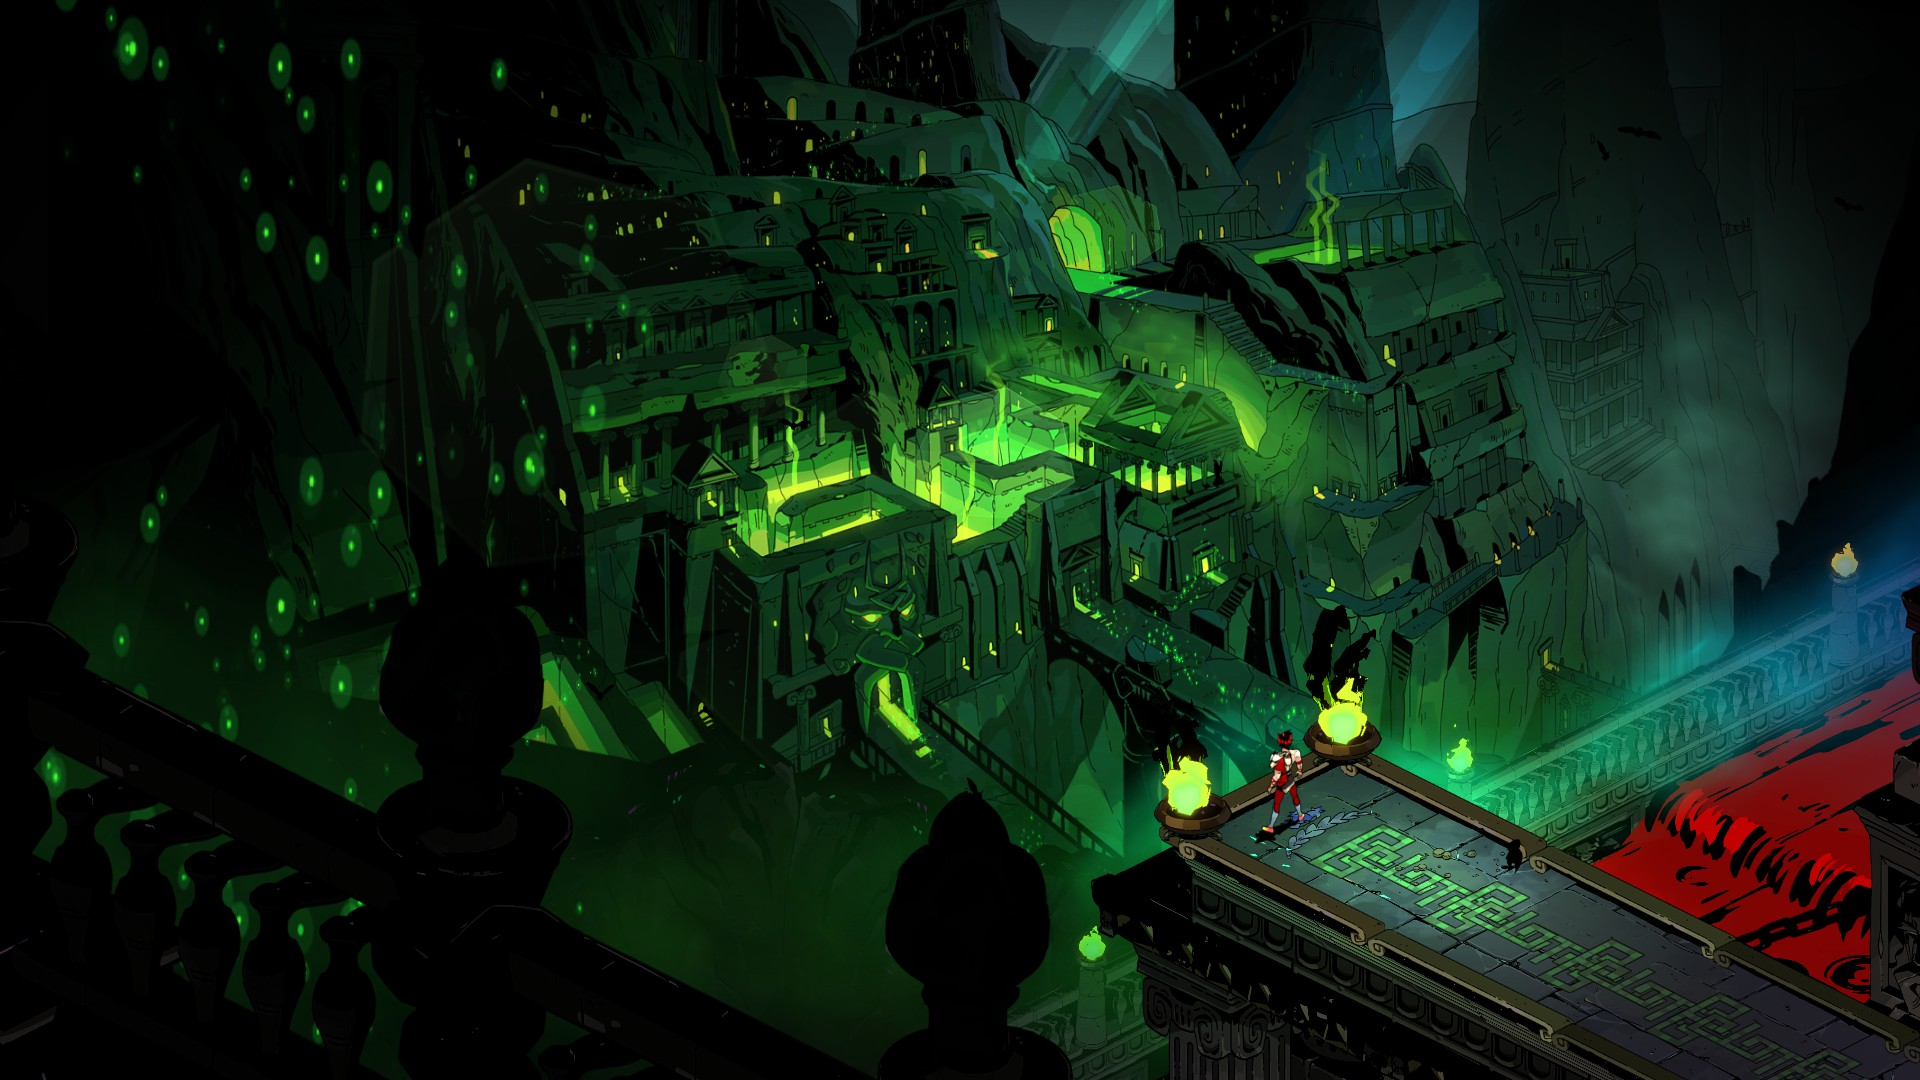
\includegraphics[width=.85\textwidth]{contenu/resources/images/hades}
    \caption[\textit{Hades} (2018), Supergiant Games]{\textit{Hades} (2018), Supergiant Games~\cite{supergiant_hades_2018}}
    \label{fig:hades}
\end{figure}

Dans ce contexte de méthodes automatisées, la génération procédurale est un procédé utilisé pour produire toutes sortes de ressources numériques~\cite{smelik_survey_2014}. Elle est en particulier utilisée pour synthétiser l'apparence visuelle des différents composants des scènes virtuelles~\cite{alessio_procedural_2021}. En combinant des méthodes algorithmiques avec de l'aléatoire, il est possible de générer des cartes de texture qui servent à habiller les mondes virtuels. Une carte de texture désigne une image qui est appliquée sur une surface pour lui donner un aspect visuel dans le but d'accentuer l'immersion des utilisateurs. Différentes textures nécessitent différentes méthodes de synthèse pour être générées. Certains genres de textures sont encore difficilement réalisables avec les méthodes existantes~\cite{lutz_cyclostationary-gaussian_2021}, notamment les textures présentant de la structure. C'est dans cette perspective que s'inscrit ce travail de recherche, qui a pour but d'approfondir notre compréhension des éléments qui constituent la structure d'une image. La compréhension d'une image et de ces éléments est le sujet d'un autre domaine, le traitement du signal (une image est un signal 2D), qui est l'étude de la manipulation et l'interprétation des signaux. Nebeker définit le traitement du signal comme étant \og [...] l'ensemble des changements appliqués aux signaux dans le but d'améliorer leur transmission et utilisation. \fg (traduction libre)~\cite{nebeker_fifty_1998}. Quand le signal étudié est une image, le domaine est appelé traitement ou analyse d'image. Afin d'obtenir une meilleure compréhension de la structure d'une image, ce travail explore l'analyse locale multirésolution et son application à la synthèse de texture procédurale. L'analyse locale multirésolution est un outil du domaine de l'analyse d'image et est détaillée dans la suite de ce manuscrit au chapitre~\ref{ch:chapitre1}. Pour décrire l'étude effectuée, ce manuscrit s'organise comme suit :

\begin{itemize}
    \item mise en contexte du sujet et introduction de concepts utiles pour la suite,
    \item explication de la théorie de Riesz et du modèle d'analyse locale multi-échelle qui en découle,
    \item application à la synthèse de texture par échantillonnage préférentiel, présentation des résultats et discussion,
    \item conclusion.
\end{itemize}
